%% example.tex
%% Jeremy Singer
%% 16 Oct 12

\documentclass{mpaper}

\usepackage{tikz}
\usetikzlibrary{fit, arrows.meta}

\usepackage{siunitx}
\usepackage[basic]{complexity}
\usepackage[super,negative]{nth}
\usepackage[linesnumbered,lined,boxed,commentsnumbered]{algorithm2e}

\usepackage{cleveref}

\usepackage[backend=bibtex,maxnames=3,maxbibnames=99,style=trad-abbrv]{biblatex}
\addbibresource{mprop.bib}

% Addendum formatting (thanks, http://tex.stackexchange.com/questions/339471/indented-addendums-using-biblatex-sourcemaps)
% Also remove doi, url since unnecessary
\DeclareFieldFormat{addendum}{}
%\DeclareFieldFormat{url}{}
%\DeclareFieldFormat{doi}{}

\usepackage{xpatch}

\xpatchbibmacro{name:andothers}{%
	\bibstring{andothers}%
}{%
	\bibstring[\emph]{andothers}%
}{}{}

\definecolor{graphc1}{RGB}{150,227,240}
\definecolor{graphc2}{RGB}{250,71,37}
\definecolor{graphc3}{RGB}{253,161,77}
\definecolor{graphc4}{RGB}{141,246,135}

\begin{document}

\title{Graph Models and Subgraph Isomorphism for Character Analysis}
\author{Kyle A. Simpson}
\matricnum{2029567}

\maketitle
%====================================================
%====================================================
\begin{abstract}
%According to Simon Peyton Jones, an abstract should address
%four key questions. First, what is the problem that this
%paper tackles? Second, why is this an interesting problem?
%Third, what is the solution this paper proposes?
%Finally, why is the proposed solution a good one?
Lorem ipsum dolor sit amet lorem ipsum dolor sit amet lorem ipsum dolor sit amet lorem ipsum dolor sit amet lorem ipsum dolor sit amet lorem ipsum dolor sit amet lorem ipsum dolor sit amet lorem ipsum dolor sit amet lorem ipsum dolor sit amet lorem ipsum dolor sit amet lorem ipsum dolor sit amet lorem ipsum dolor sit amet lorem ipsum dolor sit amet lorem ipsum dolor sit amet lorem ipsum dolor sit amet lorem ipsum dolor sit amet lorem ipsum dolor sit amet lorem ipsum dolor sit amet lorem ipsum dolor sit amet lorem ipsum dolor sit amet lorem ipsum dolor sit amet lorem ipsum dolor sit amet lorem ipsum dolor sit amet
\end{abstract}
%====================================================
%====================================================

%====================================================
\section{Introduction}
\label{sec:introduction}
%====================================================

%?? Adapt proposal introduction
Research into computer vision tasks, such as image and object recognition, is currently dominated by the use of machine learning and vector-space models, while graph encodings are comparatively less well-explored.
%Neural networks and similar machine learning constructs learn features of the inputs and data they are given, which are later used to classify or identify patterns in images or generic datasets---and have become popular due to their versatility, effectiveness and accuracy across many problem domains.
Machine learning methods apply statistical inference from training data to teach classifiers how to recognise the desired elements or features from an image---and have become popular due to their versatility, effectiveness and accuracy across many problem domains.
Vector-space models capture the area around high-contrast regions in images as salient features, or describe an image's contents in a dense and very low-level fashion.

In many cases it can be hard to reason about such models' robustness or sensitivity to different phenomena, for instance in a machine learning context these are often a function of both the training data and the model itself.
The parameters learned by these models aren't structured in a way that allows humans to easily intuit what the model has learned or to comment on the system's correctness, and it can be difficult to discern \textit{why} a particular image might be misclassified.
Recent work into \emph{adversarial images} \cite{AdversarialML} has affirmed this, given that interference can lead to classifications contrary to image content.
%Outside of this, vector-space models can represent image interest points in a way that describes their neighbourhood (or indeed, the entirety of an image), and so are easier to understand; yet they lack any way to describe the relationships between these points or to capture an object's shape.

%?? Adversarial examples in ML \cite{AdversarialML}

Graph models, long-explored in discrete mathematics, provide a simpler way of visualising problems.
Systems are broken down into \emph{vertices} and \emph{edges} between vertex pairs---capturing the relationships between objects or key features within a scene.
For many domains, this is an intuitive and effective representation, encoding rich semantics in a very natural way---which enjoys use in computational chemistry \cite{Graph-Molecules-2,Graph-Molecules-3,Graph-Molecules-1}, biology \cite{Graph-Biology-1}, and graph database analysis.
Furthermore, exact graph search and similarity metrics (e.g.\ the \emph{subgraph isomorphism} and \emph{maximum common subgraph} problems, respectively) are well-understood and an area of continual research in the field of algorithms.
%?? part of idea---need effective models to know that our similarity algorithms are a good fit?

The main aim of this paper is to explore the hypothesis that, after suitable transformation, image similarity corresponds to graph similarity according to these techniques; \cref{fig:intro-sim} gives a rough illustration of the concept.
In particular, this work focuses on character analysis and recognition, considering both the performance of graph models within a domain alongside the usefulness of any chosen analytic techniques.
By investigating these questions, this paper contributes:
\begin{itemize}
	\item A demonstration of the shortcomings of existing image graph work (\Cref{sec:image-weakness}), by attempting similarity computation on graphs built using common techniques from the literature. %given that this also requires an investigation into the effectiveness of known graph similarity techniques, this motivates the development of new models.
	This weakness motivates the development of new modelling strategies.
	\item ?? More
\end{itemize}

\begin{figure}
	\centering
	\resizebox{\columnwidth}{!}{
		\Large
		\begin{tikzpicture}
		\node[inner sep=5pt] (sagrada1) at (0,0)
		{\includegraphics[width=.35\textwidth]{images/IMG_3267.JPG}};
		\node[inner sep=5pt] (sagrada2) at (10,0)
		{\includegraphics[width=.35\textwidth]{images/IMG_3268.JPG}};
		
		\node[inner sep=5pt] (graph1) at (0,-6)
		{
			\begin{tikzpicture}
			\node[draw, circle, fill=graphc2] (n1) at (0,-1) {};
			\node[draw, circle, fill=graphc3] (n2) at (1,-0.67) {};
			\node[draw, circle, fill=graphc4] (n3) at (2,-0.33) {};
			\node[draw, circle, fill=graphc2] (n4) at (0,-2) {};
			\node[draw, circle, fill=graphc3] (n5) at (1,-1.9) {};
			\node[draw, circle, fill=graphc4] (n6) at (2,-1.8) {};
			
			\draw[<->] (n1) -- (n2);
			\draw[<->] (n2) -- (n3);
			\draw[<->] (n1) -- (n4);
			\draw[<->] (n2) -- (n5);
			\draw[<->] (n4) -- (n5);
			\draw[<->] (n5) -- (n6);
			\end{tikzpicture}
		};
		
		\node[inner sep=5pt] (graph2) at (10,-6)
		{
			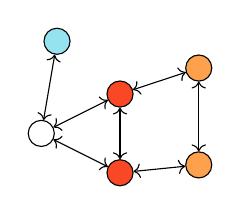
\begin{tikzpicture}
			\node[draw, circle] (n0) at (-1,-1.5) {};
			\node[draw, circle, fill=graphc1] (n7) at (-0.8,-0.33) {};
			\node[draw, circle, fill=graphc2] (n1) at (0,-1) {};
			\node[draw, circle, fill=graphc3] (n2) at (1,-0.67) {};
			\node[draw, circle, fill=graphc2] (n4) at (0,-2) {};
			\node[draw, circle, fill=graphc3] (n5) at (1,-1.9) {};
			
			\draw[<->] (n0) -- (n1);
			\draw[<->] (n0) -- (n4);
			\draw[<->] (n0) -- (n7);
			\draw[<->] (n1) -- (n2);
			\draw[<->] (n1) -- (n4);
			\draw[<->] (n2) -- (n5);
			\draw[<->] (n4) -- (n5);
			\end{tikzpicture}
		};
		
		\draw[->,thick] (sagrada1.east) -- (sagrada2.west)
		node[midway,fill=white] {Similarity};
		\draw[->,thick] (graph1.east) -- (graph2.west)
		node[midway,fill=white] {Similarity};
		
		\draw[->,thick] (sagrada1.south) -- (graph1.north)
		node[midway,fill=white] {Transform};
		\draw[->,thick] (sagrada2.south) -- (graph2.north)
		node[midway,fill=white] {Transform};
	\end{tikzpicture}
}
\caption{\textit{An example of the expected similarity between two views of the same scene. Similar objects and scenes should theoretically generate similar graphs after a suitable transformation, enabling recognition across images.}\label{fig:intro-sim}}
\end{figure}

%====================================================
\section{Graph Search and Similarity}
\label{sec:graph-search}
%====================================================

%?? Graph definitions etc
First, we must define graphs more precisely.
An undirected graph $G$ may be written $G=(V,E)$ for a vertex set $V$ and an edge set $E \subseteq \lbrace \lbrace u,v \rbrace : u,v \in V \rbrace $, i.e.\ each edge $e \in E$ is a set of two nodes from $V$.
Borrowing notation from \citeauthor{SIP-Glasgow} \cite{SIP-Glasgow}, for $u,v \in V$ we may write $u \sim_G v$ to mean $u$ and $v$ are adjacent vertices in $G$ ($\lbrace u,v \rbrace \in E$), and use $adj_G(u)$ to refer to the set of all vertices adjacent to $u$ in $G$.
Additionally, the \textit{order} of $G$ refers to the count of $G$'s vertices ($|V|$), and the \textit{size} of $G$ refers to the count of $G$'s edges ($|E|$).

?? SIP \cite{SIP-VF2, SIP-LAD, SIP-SND, SIP-Glasgow}, Regin filtering \cite{AllDiff}, Complexity \cite{Cook-SAT-SIP-NP,Computers-and-Intractibility}

?? MCS \cite{Between-MCS-SIP}, James+Ciaran+Pat's new paper too \cite{MCS-McSplit}

%====================================================
\section{On Existing Image Graph Models}
\label{sec:image-weakness}
%====================================================

\citeauthor{Plane-Graphs-From-Images} \cite{Plane-Graphs-From-Images}

?? Use existing work from proposal as basis

%====================================================
\section{The Algorithm}
\label{sec:algorithm}
%====================================================

?? Graph gen algo

?? High-level diagram, walkthrough

?? This guy's path splitting algo \cite{PathCurvature}

%====================================================
\section{Modifications to k-Down}
\label{sec:k-down-mods}
%====================================================

?? Discuss/introduce $s$-adjacency, and 3 levels of filtering

?? Keep standard filtering from supplemental graphs (adjacency matrix operates on at least 1-adjacency, exact matches are provided)

?? Could use path-based inference for new supplemental graphs, but probably way too much work for graphs of this order (i.e.\ very small)

?? Filtering at top of search---modify loop constraints, node label matching

?? Per-node of search, look at $s$-neighbourhoods

%====================================================
\section{Empirical Evaluation and Discussion}
\label{sec:evaluation}
%====================================================

?? Heatmaps per font -- examine size? font v font?

?? Matching effectiveness statistics

?? What else?

%====================================================
\section{Related Work}
\label{sec:related}
%====================================================

?? Handwriting analysis w/ kNN \cite{Graphs-Handwriting}

%====================================================
\section{Further Applications}
\label{sec:applications}
%====================================================

?? Give example of graph of two circuit diagrams here

?? Examine graph order---too big? Can we run SIP on it? How are the results?

%====================================================
\section{Conclusions}
\label{sec:conclusion}
%====================================================

?? Draw conclusions here---sum up paper.

?? Future work? Approximate GED metrics?

%====================================================
\noindent
{\bf Acknowledgments.}
%====================================================
This is optional; it is a location for you to thank people ?? TODO

%====================================================
\section{References}
%====================================================
\printbibliography[heading=none]

\end{document}